%*******************************************************************************
%*********************************** First Chapter *****************************
%*******************************************************************************

\ifpdf
\graphicspath{{Chapter1/Figs/}}
\else
\graphicspath{{Chapter1/Figs/}}
\fi

\chapter{Privacy in Bitcoin}  %Title of the First Chapter
\label{ch:Privacy in Bitcoin}
\section{Overview of Bitcoin} %Section - 1.1 
\label{sec:1-Overview of Bitcoin}
To facilitate better understanding of the issues surrounding anonymity in Bitcoin and digital currencies in general, this paper introduces a basic model of Bitcoin. For conciseness, only parts of Bitcoin that relate to anonymity are presented and the other concepts are simplified. The explanations of Bitcoin are adapted from \cite{andreas2014mastering} and \cite{narayanan2016bitcoin}.

As defined by to the creator of Bitcoin Satoshi Nakamoto, Bitcoin is a purely peer-to-peer electronic cash system that allows direct online payments without going through a financial institution \cite{Nakamoto2008}.  When a payer wants to make a payment, he constructs a \kwTransaction{}{} and broadcast it to the Bitcoin peer-to-peer network, where it can be validated by any peer (interchangeably referred to as node) through its digital signature. A simplified data structure for a \kwTransaction{}{} is shown in Fig.~\ref{fig:bitcoin_transactions}:

\begin{figure}[H]
	\begin{center}
		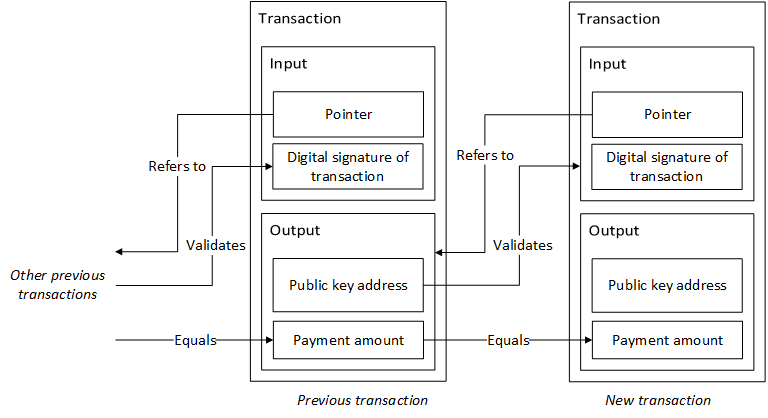
\includegraphics[scale=0.7]{bitcoin-transactions} 
		\caption{Bitcoin \textit{transactions}}
		\label{fig:bitcoin_transactions} 
	\end{center}
\end{figure}

Each \kwTransaction{}{} has a set of \kwOutput{s} which denotes public key addresses (destination of payment) and the payment amounts. For a payment to be valid, the payer must have the funds to make the payment.  The set of \kwInput{s} in a \kwTransaction{}{} denotes the source of funds used in the payment. To denote the payer’s source of funds, an \kwInput{} refers to a previous \kwOutput{} that has been paid to the public key address of the payer. Essentially a payer is using some funds that are previously paid to him/her to pay the payee. In order for the \kwTransaction{}{} to be valid, the payer must indeed own the public keys address that the previous \kwOutput{} has paid to. Nodes in the Bitcoin network validates this by checking whether the digital signature signed by the payer’s private key in the \kwInput{} is valid under the public key address in the previous \kwOutput{} referred to by the \kwInput{}. If the digital signature is valid, it means that the payer knows the private key that corresponds to the public key address that the previous \kwOutput{} has paid to, and he indeed owns the public key address. The example above shows the case where there is only one \kwInput{} and one \kwOutput{} in a transaction, but a \kwTransaction{}{} can have multiple \kwInput{s} and \kwOutput{s}. In such cases, the payer is combining sources of funds from multiple public key addresses and paying them to multiple payment addresses. At this point, it can be noted that a user can own multiple public key addresses which is achieved by simply creating them.

In addition to proof of ownership of funds, the amounts referenced by in the \kwInput{} and the amount stated in the \kwOutput{} of a \kwTransaction{}{} must also be equal. For cases where there are multiple \kwInput{s} and \kwOutput{s} in a transaction, the total amount in the previous \kwOutput{s} referenced by the \kwInput{s} must equal to the total amount stated by the \kwOutput{s}. Essentially, this means that the source of payment must be in the correct amount to fulfil the payment. Another point note is that a previous \kwOutput{} referenced by an \kwInput{} must be consumed in full, which means that the funds in the previous \kwOutput{} cannot be broken down to make a payment of an exact amount. Change is given back to the payer by creating an additional \kwOutput{} in the \kwTransaction{}{} that pays back the excess amount to one of the payer’s public key address. This mechanism ensures that the \kwInput{} and \kwOutput{} amounts of a \kwTransaction{}{} always tally. Lastly, to prevent double spending, the previous \kwOutput{} that is referenced by the \kwInput{} must not be already referenced by the \kwInput{} of another \kwTransaction{}{}.

Once a node has performed all the above checks and validated a transaction, it forwards the \kwTransaction{}{} to its neighbours who carry on the process. If the node who receives the \kwTransaction{}{} happens to be a miner node, it combines the \kwTransaction{}{} with other \kwTransaction{}{s} to form a block, and attempts to publish the \kwBlock{} to the Blockchain through the consensus protocol. The new \kwBlock{} that passes the consensus protocol is accepted by all nodes and extends the Blockchain by pointing to the latest \kwBlock{} in the Blockchain. A simplified example illustrating the relationships between \kwBlock{s} and \kwTransaction{}{s} in the Blockchain is shown in Fig.~\ref{fig:bitcoin_blockchain}.

\begin{figure}[H]
	\begin{center}
		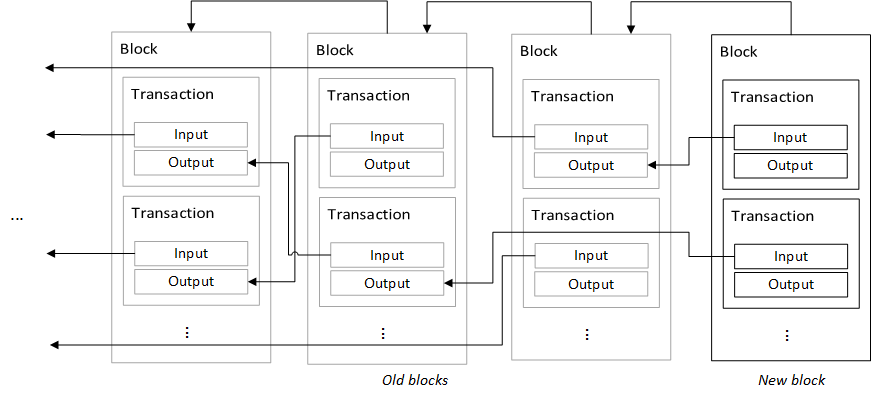
\includegraphics[scale=0.65]{bitcoin-blockchain} 
		\caption{\textit{blocks} and \textit{transactions} in the Blockchain}
		\label{fig:bitcoin_blockchain} 
	\end{center}
\end{figure}

As seen, the Blockchain contains nothing but chains of transfers of ownership of funds from the public key address in one \kwOutput{} to the public key address in another \kwOutput{} across different \kwBlock{s}. Those \kwOutput{s} that are not referred to by any \kwInput{} represent unspent funds, and can be referenced to by a new transaction.

Once a \kwTransaction{}{} has made it to the Blockchain for some while, the payment is considered confirmed.  The append-only property of the Blockchain prevents confirmed \kwTransaction{}{} from being tampered, while the public nature of the Blockchain allows anyone to check for the validity of a \kwTransaction{}{}.These features ensures that Bitcoin payments are secure. 

\section{Pseudonymity of Bitcoin}
\label{sec:1-Pseudonymity of Bitcoin}
\textbf{\textit{Pseudonymity}} refers to the case of a user using an identity that is not his/her real identity \cite{narayanan2016bitcoin}. Bitcoin achieves pseudonymity as payments made with public key addresses instead of real world identities. These addresses are generated randomly, and a user can generate as many public key addresses as he wants to further hide his/her identity. Hence it is impossible to tell who a public key address belongs to given only the information of the public key address. However pseudonymity alone in Bitcoin does not achieve privacy as public key addresses can still be linked to real world identities given other information (\S\ref{sec:1-Ways to De-anonymise Bitcoin}). Due to the public nature of the Blockchain, once a real world identity is linked to a public key address, all the \kwTransaction{}{s} in the past, present and future using that address can be linked to that real world identity.

\section{Definition of Anonymity and Anonymity Set}
\label{sec:1-Definition of Anonymity and Anonymity Set}
To achieve privacy in Bitcoin, the anonymity property needs to be satisfied. Anonymity in the context of Bitcoin requires pseudonymity and unlinkability \cite{narayanan2016bitcoin}. \textbf{\textit{Unlinkability}} refers to the case that it is hard to:

\begin{enumerate}
	\item Link different public key addresses of the same user
	\item Link different \kwTransaction{}{s} made by the same user
	\item Link a payer to the payee 
\end{enumerate}

If the above properties are satisfied, Bitcoin and digital currency systems in general can be truly anonymous and \kwTransaction{}{s} can be fully private. 

Another term that is relevant to anonymity is the \textbf{\textit{anonymity set}} \cite{narayanan2016bitcoin}. An anonymity set in Bitcoin is the set of \kwTransaction{}{s} in which an adversary cannot distinguish a particular \kwTransaction{}{} from. In other words, even if an adversary knows that a \kwTransaction{}{} is linked to a particular user, he cannot identify which \kwTransaction{}{} it is if that \kwTransaction{}{} is in its anonymity set. An anonymity set containing one \kwTransaction{}{} essentially implies no anonymity, while an anonymity set containing all the \kwTransaction{}{s} on the Blockchain implies full anonymity. Hence the size of the anonymity set in a protocol can be used to measure its level of anonymity.

\section{Ways to De-anonymise Bitcoin}
\label{sec:1-Ways to De-anonymise Bitcoin}
\subsection{Linking Payers to Payee}
\label{sec:1-Linking Payers to Payee}
Given the properties of anonymity, it can be seen that Bitcoin is not anonymous. The current Bitcoin protocol clearly violates the property that it should be hard to link a payer to the payee. The \kwInput{} of a \kwTransaction{}{} provides the link to the payer’s public key address, while the \kwOutput{} of a \kwTransaction{}{} states the payee’s public key address. For cases of direct payments without the use of an intermediary, anyone can easily tell the link between the payer and the payee since all \kwTransaction{}{s} are public on the Blockchain. 

\subsection{Linking Public Key Addresses and Transactions}
\label{sec:1-Linking Public Key Addresses and Transactions}
The other two anonymity properties apply to cases where users use different public key addresses for payments. These two properties can be violated when the different public key addresses used by the same user are linked together to form a \textbf{\textit{cluster}}. If this is achieved, then the only step left is to associate a real world identity to the cluster to fully de-anonymise the user. 

The first step of forming clusters of addresses can be achieved by inferring joint control of addresses through \textbf{\textit{shared spending}} and \textbf{\textit{shadow addresses}} \cite{Androulaki2013}. This technique is illustrated in Fig.~\ref{fig:bitcoin_cluster}.

\begin{figure}[H]
	\begin{center}
		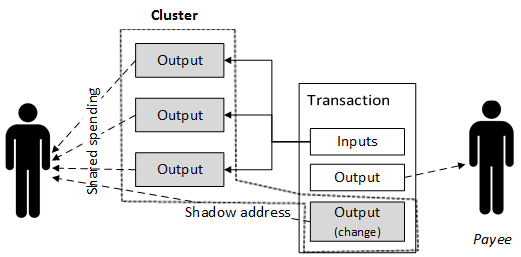
\includegraphics[scale=0.9]{bitcoin-cluster} 
		\caption{Clustering by inferring joint control of addresses}
		\label{fig:bitcoin_cluster} 
	\end{center}
\end{figure}

A \kwTransaction{}{} can contain shared spending by having multiple \kwInput{s} that refer to a different previous \kwOutput{s} (\S\ref{sec:1-Overview of Bitcoin}). One of the main reason for this kind of \kwTransaction{}{} is that the payment amount is too big to be fulfilled by any single \kwOutput{} paid to the payer and the payer has to combine funds from different \kwOutput{s} to make the payment. An adversary can make use of this spending pattern and infer that the public key addresses in the \kwOutput{s} referred to by the \kwInput{s} in a \kwTransaction{}{} belong to the same payer. In addition, a \kwTransaction{}{} often contains an \kwOutput{} that pays back the change to the payer (\S\ref{sec:1-Overview of Bitcoin}). The public key addresses in these \kwOutput{s}. referred to as shadow addresses, are in fact the addresses of payer. Hence an adversary can attempt extract these shadow addresses from a \kwTransaction{}{}.These two techniques can be used to form clusters of public key addresses that belong the same user. In the above example, the \kwOutput{s} in grey form a cluster and the public key addresses in these \kwOutput{s} belong to the Payer. Once clusters have been formed, different clusters can be linked to each other transitively as long as one public key address from each of the different clusters can be linked together. An example of this technique is illustrated in Fig.~\ref{fig:bitcoin_cluster_transitive}.

\begin{figure}[H]
	\begin{center}
		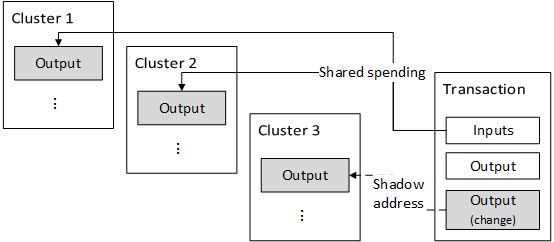
\includegraphics[scale=0.95]{bitcoin-cluster-transitive} 
		\caption{Linking clusters transitively}
		\label{fig:bitcoin_cluster_transitive} 
	\end{center}
\end{figure}

\subsection{Linking Public Key Addresses to Real World Identities}
\label{sec:1-Linking Public Key Addresses to Real World Identities}
After forming clusters of public key addresses that each belongs to a user, the last step is to assign real world identities to the clusters. This can be done by transacting with users who are targets of de-anonymization \cite{Meiklejohn2013}. Given that an adversary knows the real world identity of the user he is transacting with, he can learn one of the public key address of the user. With this one known public key address of the real world identity, a whole cluster containing that public key address can be transitively linked to the identity. Hence an adversary has the ability to attribute a list of public key addresses to a real world identity and de-anonymize the \kwTransaction{}{s} made by that identity.

\subsection{Side Channels Attacks}
\label{sec:1-Side Channels Attacks}
Side channels in Bitcoin refer to the indirect disclosure of information that can aid in the discovery of the real world identity of users. Since all \kwTransaction{}{} information such as payment amounts and timings are publicly available, an adversary can correlate \kwTransaction{}{s} patterns with other publicly available information to match \kwTransaction{}{s} to real identities \cite{narayanan2016bitcoin}. For example if activities on social media are correlated to Bitcoin \kwTransaction{}{s} activity, then social media users (assuming they are using real world identities) can be linked with the \kwTransaction{}{s} that happened during the period when they are active on social media. In addition, similar to clustering \kwTransaction{}{s} by analysing shared spending and shadow addresses, an adversary can also cluster \kwTransaction{}{s} together based on the similarities in the timings and amounts of the \kwTransaction{}{s} \cite{Androulaki2013}. The bottom-line is that as long as \kwTransaction{}{} details are public, there are always ways to make intelligent guesses about the real word identities of public key addresses.   
